\section{Vulnerability Assessment}

During the vulnerability assessment phase, we examine and analyze the information gathered during the information gathering phase. The vulnerability assessment phase is an analytical process based on the findings.

\begin{figure}
  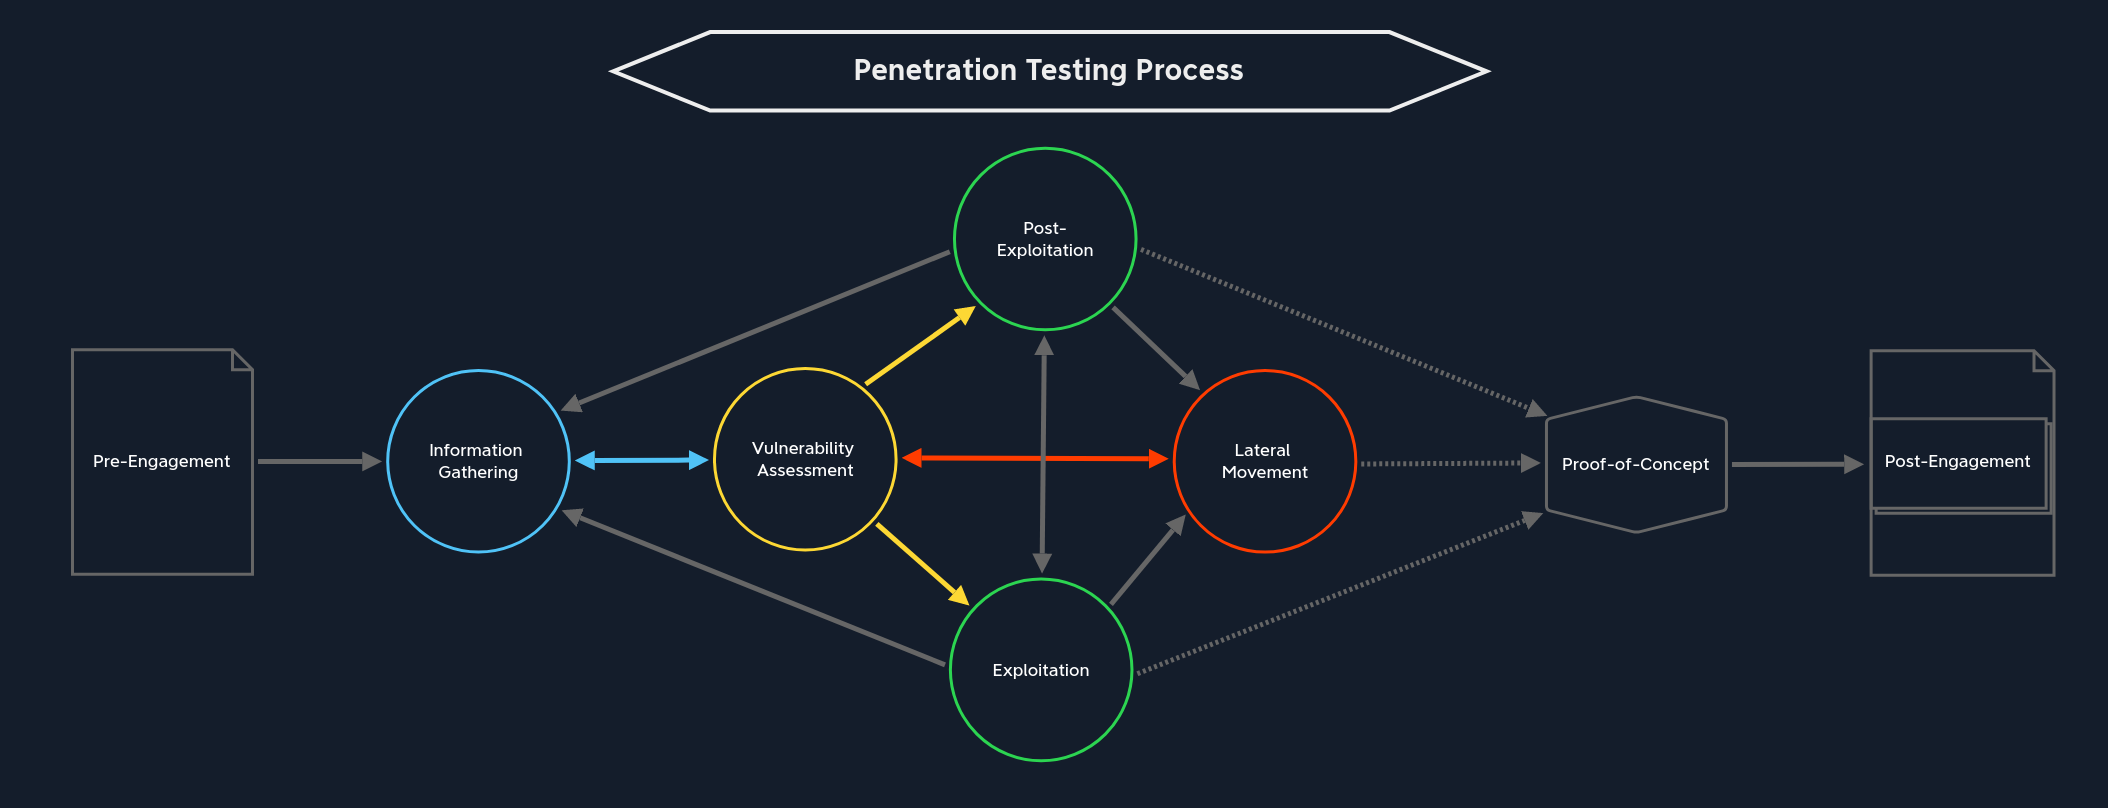
\includegraphics[width=\linewidth]{intro/process/images/vuln.png}
  \caption{Vulnerability Assessment}
  \label{fig:pentest-process-vuln-assessment}
\end{figure}

An analysis is a detailed examination of an event or process, describing its
origin and impact, that with the help of certain precautions and actions, can
be triggered to support or prevent future occurrences.

here are four different types of analysis:
\begin{itemize}
    \item {\bf Descriptive} essential in any data analysis. On the one hand, it describes a data set based on individual characteristics. It helps to detect possible errors in data collection or outliers in the data set.
    \item {\bf Diagnostic} clarifies conditions' causes, effects, and interactions. Doing so provides insights that are obtained through correlations and interpretation. We must take a backward-looking view, similar to descriptive analysis, with the subtle difference that we try to find reasons for events and developments.
    \item {\bf Predictive} 	By evaluating historical and current data, predictive analysis creates a predictive model for future probabilities. Based on the results of descriptive and diagnostic analyses, this method of data analysis makes it possible to identify trends, detect deviations from expected values at an early stage, and predict future occurrences as accurately as possible.
    \item {\bf Prescriptive} 	Prescriptive analytics aims to narrow down what actions to take to eliminate or prevent a future problem or trigger a specific activity or process.
\end{itemize}

\subsection{Vulnerability Research and Analysis}
Information Gathering and Vulnerability Research can be considered a part of
{\bf descriptive} analysis. In Vulnerability Research, we look for known
vulnerabilities, exploits, and security holes that have already been discovered
and reported. Therefore, if we have identified a version of a service or
application through information gathering and found a Common Vulnerabilities
and Exposures (CVE), it is very likely that this vulnerability is still
present.

This is where {\bf Diagnostic} analysis and {\bf Predictive} analysis is used. Once we have
found a published vulnerability like this, we can diagnose it to determine what
is causing or has caused the vulnerability. Here, we must understand the
functionality of the Proof-Of-Concept (POC) code or the application or service
itself as best as possible, as many manual configurations by administrators
will require some customization for the POC. Each POC is tailored to a specific
case that we will also need to adapt to ours in most cases.

\subsection{Assessment of Possible Attack Vectors}
Vulnerability Assessment also includes the actual testing, which is part of
{\bf Predictive} analysis. In doing so, we analyze historical information and
combine it with the current information that we have been able to find out.
Whether we have received specific evasion level requirements from our client,
we test the services and applications found locally or on the target system. If
we have to test covertly and avoid alerts, we should mirror the target system
locally as precisely as possible. This means we use the information obtained
during our information gathering phase to replicate the target system and then
look for vulnerabilities in the locally deployed system.

\subsection{The return}
Suppose we are unable to detect or identify potential vulnerabilities from our
analysis. In that case, we will return to the Information Gathering stage and
look for more in-depth information than we have gathered so far. It is
important to note that these two stages (Information Gathering and
Vulnerability Assessment) often overlap, resulting in regular back and forth
movement between them. We will see this in many videos where the author is
solving an HTB box or some CTF challenge. We should remember that these
challenges are often solved as fast as possible, and therefore speed is more
important than quality. In a CTF, the goal is to get on the target machine and
capture the flags with the highest privileges as fast as possible instead of
exposing all potential weaknesses in the system.

A (real) Penetration Test is not a CTF.

Here the quality and intensity of our penetration test and its analysis have
the highest priority because nothing is worse if our client gets successfully
hacked via a relatively simple vector that we should have uncovered during our
penetration test.



